\chapter{ACTUAL WORK}
\label{ChapterActualWork}

\section{System Architecture}

Figure~\ref{fig:architecture} gives an overview of the full RA-TFT pipeline. We broke the work into three stages, partly because it made debugging easier and partly because we wanted each stage to be independently replaceable in future iterations. Stage~1 ingests the raw five-minute CSV files for all fourteen stocks, aligns them to the NSE trading calendar, applies the cleaning steps described in Chapter~3, and stacks everything into a single long-format DataFrame. Stage~2 runs five feature extraction modules---multi-scale RV, HAR lags, jump detection, range estimators, and temporal encodings---in parallel with a GARCH fitting module and the HMM regime detector. Stage~3 takes the feature-enriched DataFrame and hands it to the TFT via PyTorch Forecasting's \texttt{TimeSeriesDataSet} abstraction. The outputs are a trained model checkpoint, per-step point forecasts, VSN importance weights, and attention maps.

\begin{figure}[h!]
\centering
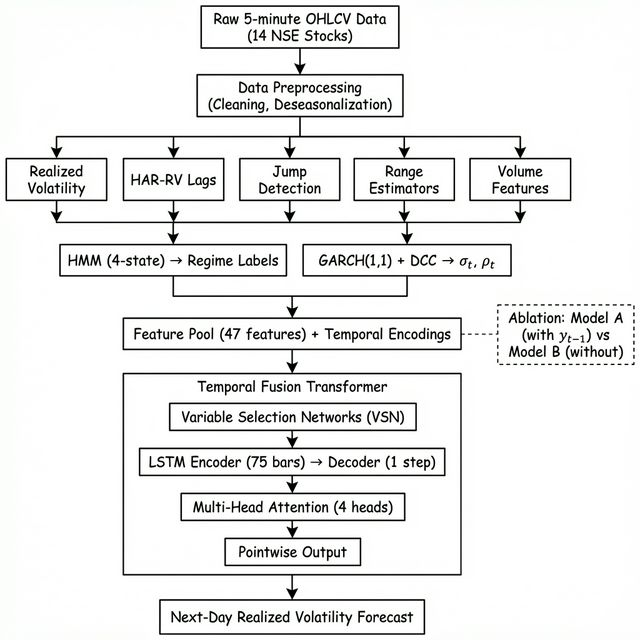
\includegraphics[width=0.78\textwidth]{Figures/system_architecture.png}
\caption{End-to-end system architecture of the Regime-Aware TFT framework.}
\label{fig:architecture}
\end{figure}

\section{Data Ingestion and Cleaning}

The practical work started with downloading historical five-minute OHLCV data for each stock and reading it into a pandas DataFrame. From there, every DataFrame was merged to a common NSE trading calendar to ensure consistent indexing across stocks. The cleaning itself involved four steps:

\begin{enumerate}
\item \textbf{Duplicate removal:} When the same timestamp appeared more than once, we kept the first row and dropped the rest. This happened occasionally due to exchange feed replays.
\item \textbf{Outlier correction:} Any bar whose absolute return exceeded ten times the 50-day rolling standard deviation was flagged as suspicious. The close price for those bars was linearly interpolated from the nearest clean neighbours on either side. In practice, fewer than 0.1\% of bars were affected.
\item \textbf{Gap filling:} Gaps of up to 12 consecutive bars (one hour) were forward-filled for OHLC and set to zero for volume. Longer gaps were left as NaN---trying to fill them would have introduced too much synthetic data.
\item \textbf{Seasonality normalization:} Each bar's squared return was divided by the historical average squared return for that particular time-of-day slot. This step removes the U-shaped intraday volatility curve, so that the model can focus on inter-day dynamics without being distracted by the mechanical opening and closing spikes.
\end{enumerate}

After cleaning, all fourteen DataFrames were concatenated with a ticker column into a single long-format table. This format is both computationally efficient and lines up exactly with how PyTorch Forecasting expects its input to be structured.

\section{Feature Extraction Modules}

All feature computations rely on vectorised pandas and NumPy operations. We deliberately avoided Python-level loops over individual bars, both for speed and to reduce the risk of off-by-one indexing bugs.

\subsection{Realized Volatility and HAR-RV Lags}

Rolling sums of squared log-returns, computed with \texttt{min\_periods} set to 90\% of the window length to handle sparse early-window observations, produce RV at four horizons. Lagged versions are generated with \texttt{pandas.Series.shift}, which is trivial but needs careful bookkeeping to avoid leaking future data.

\subsection{Jump Detection}

The code for jump decomposition is compact enough to show in full:
\begin{verbatim}
abs_ret = np.abs(log_returns)
bpv    = (np.pi/2) * (abs_ret * abs_ret.shift(1)).rolling(75).sum()
jump   = np.maximum(RV_75**2 - bpv, 0)
cont   = RV_75**2 - jump
\end{verbatim}
The bipower variation (\texttt{bpv}) uses products of adjacent absolute returns, which are robust to single-bar jumps. Taking the maximum with zero ensures the jump estimate never goes negative, which is important for numerical stability downstream.

\subsection{Range Estimators}

Parkinson, Garman-Klass, and Rogers-Satchell estimators are computed bar-by-bar directly from the OHLC columns:
\begin{verbatim}
ln_hl = np.log(df['High'] / df['Low'])
ln_co = np.log(df['Close'] / df['Open'])
parkinson = ln_hl**2 / (4 * np.log(2))
gk        = 0.5*ln_hl**2 - (2*np.log(2)-1)*ln_co**2
rs        = (np.log(df['High']/df['Close']) *
             np.log(df['High']/df['Open'])  +
             np.log(df['Low']/df['Close'])  *
             np.log(df['Low']/df['Open']))
\end{verbatim}
Each estimator captures a slightly different piece of the intrabar price path, which is why all three are included rather than picking just one.

\subsection{GARCH and Cross-Asset Module}

For each stock, a GARCH(1,1) with Student-$t$ innovations was fitted on the first 80\% of the training data using the Python \texttt{arch} package. The fitted conditional variance and standardised residuals were then broadcast from daily frequency to bar frequency. On the cross-asset side, a 20-day rolling Pearson correlation between each stock's daily return and the equally-weighted market portfolio provides a rough contagion indicator. Relative volume---defined as the current bar's volume divided by the 20-day average for that time slot---rounds out this module.

\section{Regime Detection Implementation}

The regime labels come from \texttt{hmmlearn.GaussianHMM} with full covariance matrices. We ran 200 Baum-Welch iterations for each of 10 random initialisations and kept the seed whose final log-likelihood was highest. The HMM receives two inputs: the cross-stock average daily log-return and the cross-stock average daily realized volatility. After fitting, the four latent states were sorted by their emission-mean RV so that state~0 always corresponds to ``Low'' and state~3 to ``Extreme.'' Without this sorting step, the labels would flip between runs and break downstream reproducibility. The daily regime label is then broadcast to all 75 bars of that trading day and enters the TFT as a categorical observed input.

\section{TFT Training Pipeline}

All training was done on Kaggle's free GPU instances (NVIDIA T4 or P100) using PyTorch Lightning 2.1 and PyTorch Forecasting 1.0. The main configuration choices were:

\begin{enumerate}
\item \textbf{Dataset construction:} \texttt{TimeSeriesDataSet} specifies an encoder length of 75 bars and a prediction length of 1 step, with the ticker column as the group identifier. The 47 features are assigned to the three TFT input categories: static covariates (ticker embedding), known future inputs (cyclical time features, session flags), and observed past inputs (everything else).
\item \textbf{Normalisation:} A per-stock \texttt{GroupNormalizer} with softplus transformation centres and scales each stock's target independently, so that a stock with higher average volatility does not dominate the loss.
\item \textbf{Optimiser:} Adam with an initial learning rate of 0.001 ($\beta_1=0.9$, $\beta_2=0.999$). The learning rate was halved after 5 consecutive epochs without validation improvement. Training stopped entirely after 15 epochs with no improvement.
\item \textbf{Logging:} Training and validation RMSE were logged to TensorBoard after each epoch to monitor convergence.
\end{enumerate}

\section{Ablation Study Design}

The ablation is the centrepiece of the experimental design. Two model configurations are trained with exactly the same architecture, the same hyperparameters, and the same random seed:

\begin{itemize}
\item \textbf{Model~A (with AR):} The lagged target $y_{t-1}$ is included as an observed past input. This gives the model access to yesterday's realised volatility.
\item \textbf{Model~B (without AR):} The lagged target is excluded. The model has to make do with the 47 engineered features alone.
\end{itemize}

Why bother? Because consecutive daily RV targets share 74 out of 75 constituent five-minute bars, producing a mechanical overlap of 98.7\% and a lag-1 autocorrelation of 0.9963. A model that simply parrots yesterday's number gets $R^2 \approx 0.97$ without learning anything meaningful. Stripping out the lagged target is the only honest way to measure whether the remaining features carry genuine predictive information, and that is exactly what the ablation does.

\section{Baseline Implementations}

\textbf{HAR-RV:} For each stock individually, an OLS regression with Newey-West standard errors (12 lags) was fitted on the training sample. One-day-ahead forecasts were produced on a rolling basis through the test period.

\textbf{GARCH family:} Three variants---GARCH(1,1), EGARCH(1,1), and GJR-GARCH(1,1)---were fitted per stock using the \texttt{arch} package. The variant with the lowest AIC was selected for each stock. The rolling one-day-ahead forecasting scheme was identical to HAR-RV.

\section{Tools and Technologies}

\begin{table}[!htbp]
\caption{Tools and Technologies Used}
\label{tab:tools}
\centering
\begin{tabular}{ll}
\hline
\textbf{Component} & \textbf{Tool / Library} \\
\hline
Deep learning & PyTorch 2.1, PyTorch Forecasting 1.0 \\
Training orchestration & PyTorch Lightning 2.1 \\
GARCH models & \texttt{arch} 6.2 \\
HMM & \texttt{hmmlearn} 0.3 \\
Data processing & pandas 2.1, NumPy 1.26 \\
Statistics & statsmodels 0.14, scipy 1.12 \\
Visualization & matplotlib 3.8, seaborn 0.13 \\
Compute & Kaggle (NVIDIA T4/P100) \\
Typesetting & \LaTeX{} (Overleaf) \\
\hline
\end{tabular}
\end{table}
